\documentclass[a4paper]{article}
\usepackage[english]{babel}
\usepackage[utf8]{inputenc}
\usepackage{amsmath}
\usepackage{graphicx}
\usepackage[colorinlistoftodos]{todonotes}

\title{\huge{Graphene}	\\	\LARGE{Language Tutorial} \\ \large{COMS W4115 Programming Languages and Translators}} 

\author{Adith Tekur (at2904) \\ Pooja Prakash(pk2451) \\ Sarah Panda (sp3206) \\ Sumiran Shah (srs2222) \\ Neha Rastogi (nr2477) \\ \\
Team 8}

\date{\today}


\begin{document}
\begin{figure}
\centering
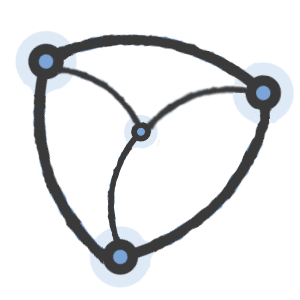
\includegraphics[width=0.3\textwidth]{logo.png}
\end{figure}
\pagenumbering{roman}

\newpage
\maketitle
\newpage
\tableofcontents
\maketitle
\pagebreak

\pagenumbering{arabic}

\section{Introduction}

Graphene aims to make graph manipulation and social network data analysis convenient using a purpose-built scripting language. The motivation for our language is the massive commonplace use of graphs and graph based data mining algorithms in today's software world. At the same time, we see a large bubble of social network and social network-like applications which manage a large backend of data which can usually be represented using a graph structure. Most of today's languages do not provide out-of-the-box or easy to use features for graph initialization, operations and management. Our language will provide this interface to be able to support generic graph algorithms as well as specific social network applications based computations on graph-like data structures.

\section{Declaration and initialization of Graphs using Graphene}


The structure of a graph data type is extermely intuitive with our language. A sample declaration of the graph is below, 
\begin{verbatim}
Graph g has d {1 <-> 2, 1 <-> 3, 1 <-> 4, 2 <-> 3, 2 <-> 4, 3 <-> 4};
\end{verbatim}
The 'd' in initializer means that the graph is directed. If it were to be an undirected graph, the declaration should begin with a 'u' instead of a 'd'.
\newline
1,2,3 and 4 in the example represent ids of nodes. Node, a derived datatype in Graphene, is used to represent an entity which can be a part of (m)any graph(s). Nodes in graphene are universal and can be declared independent of graphs. A node can be associated with 0 or more graphs. However, an edge, unlike a node, is associated with a single graph. 
\newline
\newline
In the example mentioned above, we list all the edges of the graph. Two directional edges pointing in the opposite directions and edges in undirected graphs are denoted by a $<->$ operator. A single directional edge is specified by a $->$ operator.
\newline
\newline
To declare a graph as a mesh, Graphene allows the use a simple built-in function instead of explicitely specifying all the edges. 
\begin{verbatim}
		Graph g = Graph.mesh( nodecount , type );
\end{verbatim}

\noindent An example is as follows
\begin{verbatim}
		Graph g = Graph.mesh(4, d);
\end{verbatim}
\section{Graph Operators}

We provide the basic arithmetic and logical operators. Other graph specific operators are as mentioned below.

\subsection{Edge operators '$<->$', '$->$'}
    1$<->$2 represents a bidirectional edge between nodes 1 and 2. Depending on the graph, it may also represent an undirected edge. 1$->$2 represents an edge going from node 1 to node 2. 

\subsection{Node addition operator '+'}
\begin{verbatim}
    graphObj = graphObj + graphObj.["1"];
\end{verbatim}
     
\noindent The above example shows how to add an independent node to a graph which doesnt have an edge to any other node in the graph. 

\subsection{Edge addition operator '+'}
\begin{verbatim}
	graphObj = graphObj + (graphObj.["2"] -> graphObj.["name":"John"]); 
	graphObj = graphObj + (graphObj.["1"] <-> graphObj.["name":"Bob"]);
\end{verbatim}
 
\noindent The edge addition operator is similar to the node addition operator with the difference being that the internal representation of the graph accounts for both new nodes and new edges given in the expression.
\newline
\newline

\subsection{Node removal operator}
\noindent The node removal operator is an equvalent complement to the node addition operator that is used to remove a node from a graph. An example is as follows.
\begin{verbatim}
		graphObj = graphObj - graphObj.["name":"Alice"];
\end{verbatim}

\subsection{Edge removal operator}
The edge removal operator can be used to remove an edge.
\begin{verbatim}
graphObj = graphObj - (graphObj.["2"] $->$ graphObj.["name":"John"]); 
graphObj = graphObj    - (graphObj.["1"] $<->$ graphObj.["name":"Bob"]);
\end{verbatim}


\section{Control flow}
The control flow of Graphene programs are very similar to any other programming language. The syntax of common control flow structures such as loops and conditionals are as follows.

\begin{verbatim}
if (bool)
{ 
    // matched first try!
}
else if (otherBool) 
{ 
    // that did not match, this did!
}
else 
{
    // nothing matched 
}

// foreach loops 
foreach(Node n in Graph g)
{	
}

foreach(Edge n in Graph g)
{
}

// for loops 
for (i = 0; i < 10; i++)
{
}

// while loops 
while (bool)
{
}
\end{verbatim}

\section{Library Functions}
\label{sec:examples}

Graphene provides multiple standard graph operations as library functions. This list covers them and explains the usage and outcome of the functions.

\subsection{Graph object methods}

\begin{verbatim}isDirected()\end{verbatim} Returns a boolean value indicating if the object represents a directed or an undirected graph.
\newline

\begin{verbatim}getNode(["id"])\end{verbatim} Returns the node object from the graph which matches the node id.
\newline
\begin{verbatim}getNode(["key":"value"])\end{verbatim} Returns the first node object (lowest id value) which satisfies the key-value pair mapping.
\newline
\begin{verbatim}hasNode(["id"])\end{verbatim} Returns a boolean value indicating if the graph has a node matching the node id.
\newline
\begin{verbatim}hasNode(["key","value"])\end{verbatim} Returns a boolean indicating if the graph has a node matching the key-value pair predicate.
\newline
\begin{verbatim}hasEdge(["id"] edgeOp ["id"])\end{verbatim} Returns a boolean indicating if there exists an edge which connects two nodes matching the node-ids. $<$edgeOp$>$ can be either $->$ or $<->$ indicating a directed or undirected edge.
\newline
\begin{verbatim}hasEdge(["key","value"] edgeOp ["key","value"])\end{verbatim} Similar to the above function, but matches nodes based on key-value pairs rather than id.
\newline
\begin{verbatim}addNode(["key":"value", "key":"value" , "key":"value"])\end{verbatim} Adds a new node to the graph and initializes its data with the given key-value pairs. If an id is not specified, it auto-generates the next available one.
\newline
\begin{verbatim}deleteNode(["id"])\end{verbatim} Deletes the node having the specified id from the graph.
\newline
\begin{verbatim}getDFS(Node root)\end{verbatim} Returns a DFS tree generated from the graph with the specified node as the root of the tree.
\newline
\begin{verbatim}getBFS(Node root)\end{verbatim} Returns a BFS tree generated from the graph with the specified node as the root of the tree.
\newline
\begin{verbatim}cluster(lambda expr)\end{verbatim} Returns a list of lists of node ids which are clusters formed by running the lambda expression over each pair of nodes in the graph. The lambda function supplied by the user should return a boolean value indicating if two nodes belong to the same cluster.
\newline
\begin{verbatim}mergeWith(graph, lambda expr)\end{verbatim} Returns a single graph which is a combination of both the graphs. The lambda expression takes in two nodes, one from each graph and returns a boolean value indicating if they are to be merged.
\newline

\subsection{Node object methods}

\begin{verbatim}inDegree()\end{verbatim} Returns the in-degree (number of edges pointing to the node) of the node object.
\newline
\begin{verbatim}outDegree()\end{verbatim}Returns the out-degree (number of edges originating from the node) of the node object.
\newline
\begin{verbatim}degree()\end{verbatim}Returns the sum of in-degree and out-degree for directed graphs and the in-degree ( = out-degree) for undirected graphs.
\newline
\begin{verbatim}listAdjacent()\end{verbatim} Returns a list of nodes which are adjacent to the object node. That is, there exists an edge pointing from the object node to the adjacent nodes.
\newline
\begin{verbatim}listNotAdjacent()\end{verbatim}Returns the complement of the above function
\newline

\section{Sample Programs}

The following programs demonstrate different ways to use Graphene to manipulate and extract valuable information from graphs. We begin with a simple “Hello World” application that does the simplest operation of declaring a graph and adding a new edge to it.

\subsection{Hello World}

\begin{verbatim}
$g has d {1<->2, 2->3, 4->3};
print("Hello World. The graph you defined has " + g.listNodes().count()
+ " Nodes and "+ g.listEdges().count()+ " Edges");
\end{verbatim}

\noindent This is a simple Hello World program. The first statement declares and initialises a directed graph named $g$ with nodes 1, 2, 3 and 4, and edges represented by the arrows between the nodes. The second statement prints “Hello World..” along with the number of nodes and edges in the graph found using the built-in functions for a Graph object.
\newline

\subsection{Create a network, identify all the closely-knit groups and find who the go-to person in each group}

\begin{verbatim}
def ($G) => findMostInfluential
{ 
  // By default it returns the strongly connected component 
  $Subgraphs = Cluster($G, lambda membership($node1, $node2) :
  this.hasEdge($node1, $node2));
  foreach($graph in $Subgraphs) 
  {
    $maxdegree=0; 
    $influential = $graph[0]; 
    foreach($user in $graph.getNodes())
    { 
      $degree = indegree($graph,$user) 
      if $maxdegree < $degree
      {
        $maxdegree = $degree; 
        $influential = $user; 
      } 
    } 
    $Minfluential.add($influential); 
  }
} => ($Minfluential) 


$g has d {1->2,3->5,2->5,3-4}; 
$gotoperson = findMostInfluential ($g); 
print("Found "+ gotoperson.length() + "Closely-Knit groups"); 
plot($g, highlight(gotoperson));
\end{verbatim}

\noindent This program demonstrates how to find the most influential person in a social network. The influence of a person is defined in terms of the number of other people in the network that know him/her. In order to do so, in the above example, we first declare a graph and push the job of finding the groups within the network and most influential person in each group to the function named $findMostInfluential()$.  
\newline\newline
This function takes in the graph object as its argument and clusters the nodes into groups based on a user defined lambda function that decides how the cluster function should work. The clusters are in turn graphs and hence, for each of the clusters, the node with the highest indegree (number of incoming edges that can be found using the built-in function $indegree()$) is determined to be the most influential person of the group. The output of the program is the number of clusters in the network that meet the user defined criteria, and also a visualization of the graph with the most influential people highlighted.
\newline

\subsection{Given a node representing a url, generate a graph of other web-page nodes which carry a common characteristic (for example websites that allow google adsense), that is defined by a lamda function}

\begin{verbatim}


def ($lambda,$url) => SearchBot 
{
    $connections=d{};
    $connections = $connections + connections.["url":url];
    
    /*
    Queue data structure is assumed to be implemented already
    for simplicity
    */
    
    $url_list = Queue();
    $url_list.push($url);
    while ($url_list.length()!=0)
    {
        $c_url = $url_list.pop();
        
        /* 
        user defined function to parse the contents
        of the page and extract the links
        */
        
        links = getlinksfromHTMLcontents($c_url);
        foreach ($link in $links)
        {
            if($lambda($url)==True)
            {
                $url_list.push($link);
                $connections = $connections + $connections.[$link];
                $connections = $connections + 
                ($connections.[$c_url] -> $connections.["url":$link]);
            }
        }
    }
} => ($connections)

\end{verbatim}

\noindent This program demonstrates how to search for a set of nodes within graphssuch that the seleceted nodes satisfy a certain predicate. It takes two input parameters - an initial URL and a lambda which is a predicate to determine if a node satisfies a condition. It continually parses the contents of the input URL and searches for nodes that satisfy the predicate. Everytime such a node is found, it is added to $connections$ which is finally returned.
\newline

\subsection{Given two different social network graphs and a user who is new to one of the networks, build a recommendation system that tells the user who all on this new network he might now, by analysis of overlap of the two networks}

\begin{quote}
\begin{verbatim}
def ($OldGraph, $NewGraph, $user) => WhoYouMayKnow
{
    $OldFriends = $user.listAdjacent();
    $Suggestions = [];
    foreach ($friend in $OldFriends)
    {
        if ($NewGraph.hasNode($friend["id"]) == True and 
        	$NewGraph.hasEdge($user["id"]-> $friend["id"]) == False)
        {
        	$Suggestions.append($friend);
        }
    }
} => ($Suggestions)
\end{verbatim}
\end{quote}

\noindent This code snippet shows a user defined function which takes in three parameters - one graphs objects representing the old graph, one new graph and a node representing the user.
$user.listAdjacent()$ returns a list of nodes which are nodes pointed to by it. An empty node list called $Suggestions$ is created.
The $OldFriends$ list is iterated and each element is added to the Suggestions list if it does not already exist. The Suggestions list is then returned.
\newline

\subsection{Find the minimum set of nodes in a network that have global reach. A node's reach is defined as all its adjacent nodes.}

\begin{quote}
\begin{verbatim}
def ($graph) => GlobalReach
{
    $Nodes = [];
    while($graph.listNodes().length()!=0){
    
     $current = getNodeWithMaxDegree($graph);
     $Nodes.append($current);
     foreach($temp in $graph.listAdjacent($current)){
      $graph = $graph - $graph.[$temp["id"]];
     }
     $graph = $graph - $graph.[$current["id"]];
    }
} => ($Nodes)

def ($graph) => getNodeWithMaxDegree 
{
  $maxnode = $graph.getNodes()[0];
  $maxdegree = $graph.getAdjacent($maxnode).length();
  foreach($node in $graph.getNodes())
  {
    $curr = $graph.getAdjacent($node).length();
    if($curr > $maxdegree)
    {
      $maxnode = $node;
      $maxdegree = $curr;
    }
  }
} => ($maxnode)
\end{verbatim}
\end{quote}

\noindent This function takes in a graph and returns the list of minimum nodes with global reach. In the above example, the reach of a node is the set of its adjacent nodes. The criteria, however, is not rigid and the flexibility can be achieved with the use of appropriate lambda functions. A greedy approach is used in the above example where in every iteration, a node with the highest degree is found and its adjacent nodes are removed from the nodes. The node is added to the final list and is then removed from the graph using simple graph operations. This modified graph is then used for the next iteration until the graph becomes empty.
\newline

\section{Executing a Graphene program}

Graphene is interpreted and is very simple to execute. Graphene source files conventionally end in a ".ene" extension. If a source file with no extension is specified, the compiler will still try to interpret it as a plain-text file containing graphene source code.

The Graphene interpreter can be summoned by "graphene" followed by the source file name.

eg: Consider a source file called "graph.ene". It can be run by:

\begin{verbatim}
$ graphene graph.ene
Hello, World!
$
\end{verbatim}



\end{document}